\chapter{Optimización Inteligente}
Planificación y Scheduling representa un área de gran relevancia en Inteligencia Artificial. Muchos problemas reales se modelan como problemas de P\&S.

La \textbf{planificación} es un proceso de deliberación que \ul{escoge y organiza acciones anticipando sus resultados o consecuencias}.

Lo \textbf{scheduling} es un proceso de \ul{asignación de recursos a tareas sobre el tiempo para optimizar uno o más objetivos}.

\begin{figure}[htbp]
   \centering
   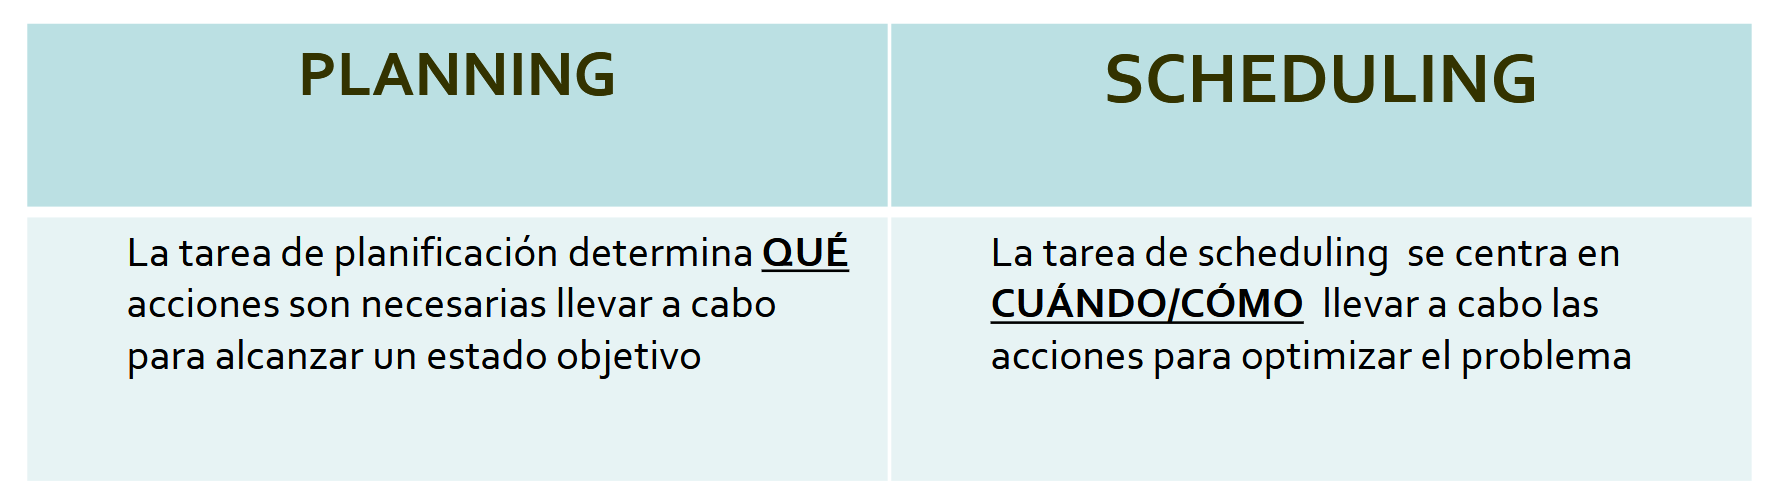
\includegraphics{images/04/PS.png}
   \caption{P\&S}
   \label{fig:04/PS}
\end{figure}
\section{Scheduling}
Un problema de scheduling consiste en organizar en el tiempo un
conjunto de actividades que compiten por el uso limitado de recursos


\subsection{JSP}
JSP stands for Job-Shop Scheduling, y es un paradigma de los problemas de scheduling es muy simple de
enunciar y muy difícil de resolver.

\begin{paracol}{2}
   \colfill
   \begin{itemize}
      \item $n$ trabajos cada uno compuesto por un conjunto ordenado de tareas
      \item $m$ maquinas donde se procesan las tareas
      \item Cada tarea debe ser procesada en una única máquina durante un tiempo determinado y en un orden prefijado;
      \item El objetivo es minimizar \textit{makespan}: instante de finalización de la última tarea
   \end{itemize}
   \colfill
   \switchcolumn

   \begin{itemize}
      \item \textbf{Datos} - $p_{ij}$ es el tiempo de proceso de la tarea i en el trabajo j;
      \item \textbf{Variables} - $st_{ij}$ es el tiempo de inicio de tarea i en el trabajo j;
      \item \textbf{Restricciones} -
      \begin{itemize}
         \item Secuential - $st_{ij} + p_{ij} \leq st_{i(j+1)}$
         \item Capacidad - $st_{ij} + p_{ij} \leq st_{kl} \bigvee st_{kl} + pkl \leq st_{ij}$
         \item Sin interrupción - $Cij = st_{ij} + p_{ij}$
      \end{itemize}
      \item \textbf{Objetivo} - Construir una ordenación de las tareas en el tiempo de manera que
      se satisfagan todas las restricciones sobre cada máquina.

      \begin{itemize}
         \item Mimimize the makespan: $C_{max} = max C_{ij}$
         \item Minimize total flow time: $C_{sum} = \sum C{i}$
         \item Minimize makespan + energy
      \end{itemize}
   \end{itemize}

\end{paracol}

\subsection{CSP - Constraint Satisfaction Problem}
{Muchos problemas pueden ser expresados mediante:\ns
\begin{itemize}
	\item Un conjunto de variables.
	\item Un dominio de interpretación (valores) para las variables.
	\item Un conjunto de restricciones entre las variables.
   \item La solución al problema es una asignación válida de valores a las variables.
\end{itemize}}

\note{Formalization omitted here}

En general, los problemas de optimización son particularmente difíciles de resolver.
En general, basta con una \ul{solución razonablemente buena} (factible, optimizada, pero no la
óptima) \ul{en un tiempo razonable}, y si puede obtener con métodos aproximados (como alternativa a los métodos exactos), cómo la \textbf{Búsqueda Heurística} / Metaheurística:\\
 La solución es obtenida (generada / mejorada), mediante un proceso de búsqueda en un amplio espacio de estados/soluciones.
Hay tambien \textbf{técnicas inferenciales}, que no se sostituyen por la búsqueda, sino que la complementan. Estas técnicas son utilizadas para \ul{reducir el espacio de búsqueda}, y se basan en la \textbf{lógica} y en la \textbf{teoría de conjuntos}.
Conociendo las consecuencias de una acción, podemos reducir el espacio de búsqueda, y por lo tanto, la complejidad del problema.

\begin{itemize}
   \item Búsqueda Local (Local Search) - Se parte de una solución inicial y se busca una solución mejor en el vecindario de la solución actual.
   \item Búsqueda Sistemática (Systematic Search) - Se parte de una solución inicial y se busca una solución mejor en todo el espacio de soluciones.
\end{itemize}

\begin{itemize}
   \item Métodos Constructivos - Construyen una solución paso a paso, añadiendo o eliminando elementos de la solución.
   \item Métodos de Mejora - Parten de una solución inicial y la mejoran iterativamente mediante movimientos locales.
   \item Métodos Evolutivos - Combinan soluciones previas
\end{itemize}


\subsection{Algoritmo Genéticos}
Los \textbf{algoritmos genéticos} son un tipo de algoritmo evolutivo que se utiliza para encontrar soluciones aproximadas a problemas de optimización y búsqueda. Estos algoritmos reflejan el proceso de selección natural en la evolución de las especies, y se basan en la idea de que las soluciones a un problema pueden ser representadas como individuos en una población, y que la evolución de la población puede conducir a la generación de soluciones cada vez mejores.

\begin{table}[htbp]
\centering
\begin{tabular}{|p{4cm}|p{4cm}|p{4cm}|p{4cm}|}
\hline
\textbf{Término GA} & \textbf{Explicación} & \textbf{Término Optimización} & \textbf{Explicación equivalencia} \\
\hline
Medio o entorno & Lugar en el que se desempeñan los individuos & Problema & El individuo se desenvuelve en un entorno, que determina cómo puede actuar. En ese caso, este marco es el problema. \\
\hline
Individuo & Representa a un individuo de la población que compite con otros & Solución & Nuestros individuos son las soluciones al problema, aquello que queremos gradualmente evolucionar hacia mejores individuos o soluciones. \\
\hline
Cromosoma o genotipo & Es la forma en la que se representa internamente un individuo & Codificación de la solución & Representa cómo representamos internamente la solución (pueden haber diferentes). \\
\hline
Gen & Es una de las partes atómicas del cromosoma & Variable de decisión & Representa una decisión atómica en el problema. \\
\hline
Alelo & Son los valores que puede tomar un gen & Dominio de la variable & Si un gen es equivalente a una variable de decisión, el alelo representa su dominio. \\
\hline
Fenotipo & Representan la representación externa del individuo o solución, que es lo que al final es evaluado en el medio. A veces puede ser equivalente al genotipo. & - & - \\
\hline
Función de fitness & Determina el desempeño del fenotipo de un individuo en el entorno & Función objetivo & Equivalente, se usa simplemente diferente terminología. \\
\hline
\end{tabular}
\caption{Equivalencia entre términos de Algoritmos Genéticos y Optimización}
\end{table}


\begin{paracol}{2}

   \colfill
   La operación fundamental es la \textbf{cruce}, que toma n padres (típicamente 2) y generar m hijos (típicamente 2);
   consiste en heredar material genético
   de los padres.
   La \ul{asunción} es que si los padres tienen buen material genético, la mezcla del material genético de ambos también será buena.\\
   Entonces, el efecto de la cruza es \textit{explorar} el espacio de búsqueda con \textbf{material prometedor}.
   
   La operación de \textbf{mutación} es una operación que se aplica a un individuo y cambia aleatoriamente uno o más genes de ese individuo. Corisponte a una búsqueda local, porque sólo se cambia un gen a la vez, y entonces el hijo serà cerca de su padre.
   \colfill
   
   \switchcolumn

   \begin{figure}[htbp]
      \centering
      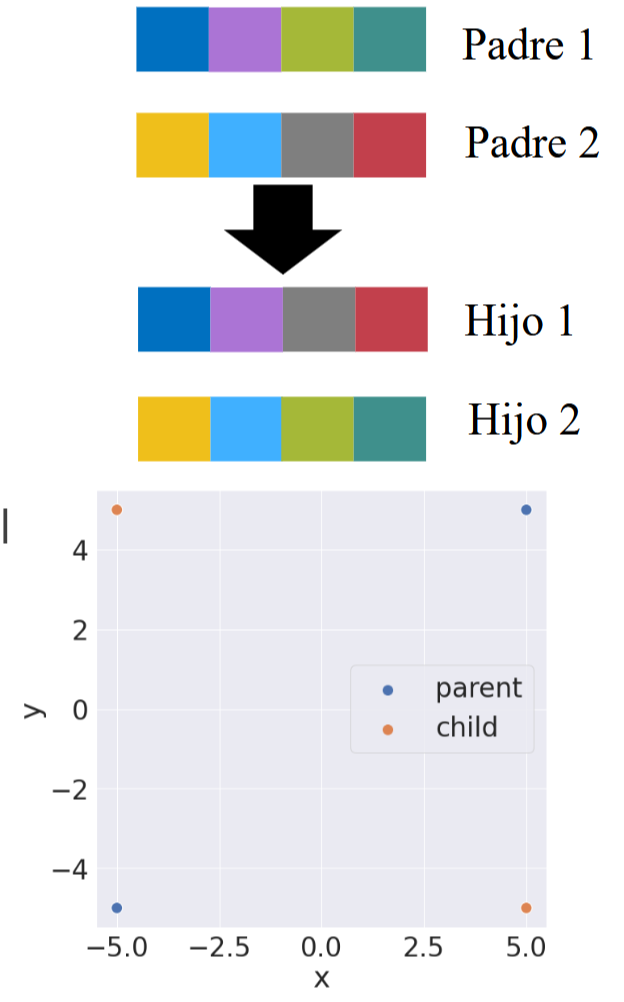
\includegraphics[width=0.48\columnwidth]{images/04/cruce.png}
      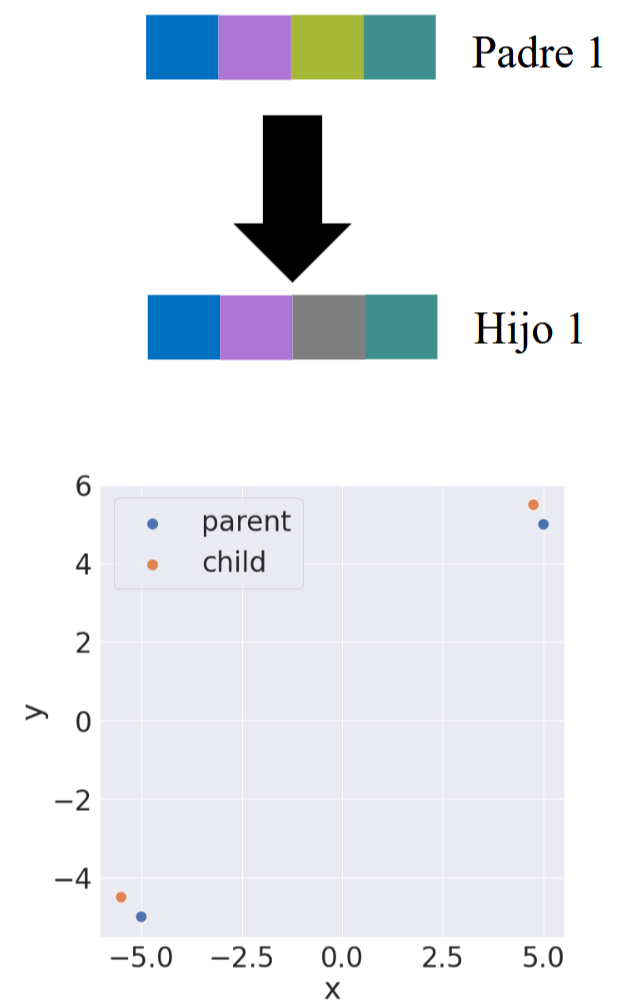
\includegraphics[width=0.48\columnwidth]{images/04/mutacion.png}
      \caption{Cruce y mutación}
      \label{fig:04/cruceYMutacion}
   \end{figure}
\end{paracol}

TODO selección des padres
TODO criterio de parada

\subsubsection{Resumen}
\begin{enumerate}
	\item Una \textbf{representación} adecuada de las \textit{soluciones} del problema (individuos).\\
   Cromosomas, genes, genotipo, fenotipo.
	\item Una forma de crear una \textit{\textbf{población} de soluciones inicial} (individuos iniciales). A
menudo, aleatoria.
	\item Una \textbf{función de evaluación} capaz de medir la adecuación de cualquier solución
	(individuo) al problema. Fitness.
	\item Un conjunto de \textbf{operadores evolutivos} para combinar las soluciones existentes con el
objetivo de obtener nuevas soluciones (nuevos individuos): \textit{selección}, \textit{cruce}, \textit{mutación} y \textit{reemplazo} de individuos. Guían el proceso de la búsqueda.
	\item Conjunto de \textbf{parámetros de entrada}: tamaño de la población, número de iteraciones
	(generaciones), probabilidades de selección, etc.
\end{enumerate}


Podemos resumir el proceso de un algoritmo genético en los siguientes pasos:
\begin{enumerate}
	\item \textbf{Codificación} de Soluciones/instanciaciones.
	\item \textbf{Población Inicial}:
	\begin{enumerate}
      \item Generar población aleatoria de n individuos: {x} (posibles soluciones del problema)
      \item Evaluar la aptitud o fitness f(x) de cada individuo.
   \end{enumerate}
	\item \textbf{Ciclo-Generacional}:
	\begin{enumerate}
   	\item \textbf{Selección} Seleccionar dos padres de la población de acuerdo a su aptitud:
Probabilidad de cruce (pc).
	\item \textbf{Cruce} Combinar los genes de los dos padres para obtener descendientes.
	\item \textbf{Mutación} Con una probabilidad de mutación (pmut ), mutar cada gen de los
cromosomas hijo.
	\item \textbf{Reemplazo} Añadir nuevos hijos y determinar nueva población.
   \end{enumerate}
	\item Verificar condición de parada:
	\begin{enumerate}
   	\item \textbf{Parada}: proporcionar como solución el individuo con mejor valor de aptitud f(x).
	\item \textbf{Ciclo}: Ir al paso 2
   \end{enumerate}
\end{enumerate}